\chapter{Formulas}\label{ch:formulas}

This chapter lists all formulas which are derived from the binormal model to this model with an additional normal.
All formulas listed are either tested by using a \gls{cas}
and calculating the integrals analytically with ranges $-\infty$ to $\infty$ or
using the quadrature procedure with large enough ranges such that the error is (numerically) zero.
Those two procedures are explained in \cref{ch:intsympy}.

\section{Definition of the trinormal distribution, \texorpdfstring{$P_{tmg}$}{P tmg}}
\label{sec:definition-of-the-trinormal-distribution-p_tmg}

We would like to add a third normal to the already existing two trivariate normals,
which is placed right in the middle between those two.
For our proposed mixture of normals we then have
\begin{align}
	\label{eq:normal_mix_pdf}
	P_{tmg}(w, \theta_l, r_t)
	= \alpha (1-\delta) \mathcal{N}(\mu_1, \Sigma_1)
	+ (1-\alpha) (1-\delta) \mathcal{N}(\mu_2, \Sigma_2)
	+ \delta \mathcal{N}(\mu_3, \Sigma_3),
\end{align}
where $\mathcal{N}$ denotes the multivariate normal distribution,
$\alpha \in (0,1)$ is the mixture fraction of the binormal,
and $\delta \in [0,1)$ is the weight of the third normal.
The mean vectors and the covariance matrices are defined in the following.

We define the mean vectors of the first
and second normal distributions as $\mu_1 = (w_1, \theta_{l1}, r_{t1})^\top$,
and $\mu_1 = (w_2, \theta_{l2}, r_{t2})^\top$,
where $w_1 > w_2$ (due to a convention in the code) and the covariance matrices as
\begin{align}
	\Sigma_1 =
	\begin{pmatrix}
		\sigma_w^2 & 0                                                      & 0                                                      \\
		0          & \sigma_{\theta_{l1}}^2                                 & \rho_{\theta_l r_t} \sigma_{\theta_l 3} \sigma_{r_t 3} \\
		0          & \rho_{\theta_l r_t} \sigma_{\theta_l 3} \sigma_{r_t 3} & \sigma_{r_{t1}}^2
	\end{pmatrix},
	\text{ and }
	\Sigma_2 =
	\begin{pmatrix}
		\sigma_w^2 & 0                                                      & 0                                                      \\
		0          & \sigma_{\theta_{l2}}^2                                 & \rho_{\theta_l r_t} \sigma_{\theta_l 3} \sigma_{r_t 3} \\
		0          & \rho_{\theta_l r_t} \sigma_{\theta_l 3} \sigma_{r_t 3} & \sigma_{r_{t2}}^2
	\end{pmatrix}.
\end{align}
It might be of interest that there is no correlation between $w$ and $\theta_l$ or $w$ and $r_t$.
That is to make the \glspl{pdf} mathematically more tractable which also makes the \gls{pdf} family less general.
This is not the case for the third normal, though.

It has already been said,
that we would like to place the third normal right at the mean,
therefore $\mu_3$ and $\Sigma_3$ are defined as
\begin{align}
	\mu_3 =
	\begin{pmatrix}
		\overline{w}        \\
		\overline{\theta_l} \\
		\overline{r_t}
	\end{pmatrix},
	\text{ and }
	\Sigma_3 =
	\begin{pmatrix}
		\sigma_{w 3}^2 &
		\rho_{w \theta_l 3} \sigma_{w 3} \sigma_{\theta_l 3} &
		\rho_{w r_t 3} \sigma_{w 3} \sigma_{r_t 3} \\
		\rho_{w \theta_l 3} \sigma_{w 3} \sigma_{\theta_l 3} &
		\sigma_{\theta_l 3}^2 &
		\rho_{\theta_l r_t 3} \sigma_{\theta_l 3} \sigma_{r_t 3} \\
		\rho_{w r_t 3} \sigma_{w 3} \sigma_{r_t 3} &
		\rho_{\theta_l r_t 3} \sigma_{\theta_l 3} \sigma_{r_t 3} &
		\sigma_{r_t 3}^2
	\end{pmatrix}.
\end{align}
The advantage over just two normal \glspl{pdf} is that
we can now express a greater variety of shapes.
We also define some additional relationships for this third normal distribution.
\begin{align}
	\label{eq:lambda}
	\lambda_w \equiv \frac{\sigma_{w 3}^2}{\wptwo}, \quad
	\lambda_\theta \equiv \frac{\sigma_{\theta_l 3}^2}{\thlptwo}, \quad
	\lambda_r \equiv \frac{\sigma_{r_t 3}^2}{\rtptwo},
\end{align}
\begin{align}
	\label{eq:lambda_two}
	\lambda_{\theta r} \equiv
	\frac{\rho_{\theta_l r_t} \sigma_{\theta_l 3} \sigma_{r_t 3}}{\rtpthlp}, \quad
	\lambda_{w \theta} \equiv
	\frac{\rho_{w \theta_l} \sigma_{w 3} \sigma_{\theta_l 3}}{\wpthlp}, \quad
	\lambda_{w r} \equiv
	\frac{\rho_{w r_t} \sigma_{w 3} \sigma_{r_t 3}}{\wprtp}.
\end{align}
Hence, we can rewrite $\Sigma_3$ as
\begin{align}
	\Sigma_3 =
	\begin{pmatrix}
		\sigma_{w 3}^2 &
		\wpthlp \cdot \lambda_{w \theta} &
		\wprtp \cdot \lambda_{w r} \\
		\wpthlp \cdot \lambda_{w \theta} &
		\sigma_{\theta_l 3}^2 &
		\rtpthlp \cdot \lambda_{\theta r} \\
		\wprtp \cdot \lambda_{w r} &
		\rtpthlp \cdot \lambda_{\theta r} &
		\sigma_{r_t 3}^2
	\end{pmatrix}.
\end{align}

\section{Normalized Variables}\label{sec:normvars}

Since \gls{CLUBB} is mostly using \enquote{normalized variables},
we are going to list those, which are given in standard form.
\begin{align}
    \tilde{\theta}_l'
    &\equiv \frac{\theta_l - \overline{\theta_l}}{\sqrt{\overline{\theta_l'^2}}}\frac{1}{\sqrt{\frac{1 - \delta \lambda_\theta}{1 - \delta}}}, \label{eq:theta_l_prime_tilde}
\end{align}
\begin{align}
    \tilde{r}_t'
    &\equiv \frac{r_t - \overline{r_t}}{\sqrt{\overline{r_t'^2}}}\frac{1}{\sqrt{\frac{1 - \delta \lambda_r}{1 - \delta}}}, \label{eq:r_t_prime_tilde}
\end{align}
where $\overline{\theta_l}$ and $\overline{r_t}$ are the means for the full summed up \gls{pdf}
and $\overline{\theta_l'^2}$ as well as $\overline{r_t'^2}$ are the variances for $\theta_l$ and $r_t$.
\begin{align}
    \tilde{\sigma}_w
    &\equiv \frac{\sigma_w}{\sqrt{\overline{w'^2}}}
    \frac{1}{\sqrt{\frac{1-\delta\lambda_w}{1-\delta}}}, \label{eq:sigma_w_tilde}
\end{align}
\begin{align}
    \tilde{\sigma}_{\theta_l i}
    &\equiv \frac{\sigma_{\theta_l i}}{\sqrt{\overline{\theta_l'^2}}}
    \frac{1}{\sqrt{\frac{1-\delta\lambda_\theta}{1-\delta}}}, \label{eq:sigma_theta_l_i_tilde}
\end{align}
\begin{align}
    \tilde{\sigma}_{r_t i}
    &\equiv \frac{\sigma_{r_t i}}{\sqrt{\overline{r_t'^2}}}
    \frac{1}{\sqrt{\frac{1-\delta\lambda_r}{1-\delta}}}. \label{eq:sigma_r_t_i_tilde}
\end{align}

%\section{Transformation of the equations}\label{sec:transformationequations}

Having established the definition of the sum of normal distributions in \cref{sec:def_trinormal}
to enhance mathematical tractability,
we now delve into the transformation of equations from the existing binormal representation
used in CLUBB-SILHS\autocite{larson2022clubbsilhs} to a trinormal one.
While the formulas for the binormal case are well-defined (see~CLUBB-SILHS\autocite{larson2022clubbsilhs}),
the simplicity of the means and standard deviations employed in the trinormal representation suggests
the existence of a specific transformation that holds true.
This chapter will demonstrate that the following transformations,
denoted by the subscript \enquote{dGn} for the binormal case,
successfully achieve this conversion.
\begin{align}
    \overline{w'^2} \frac{1 - \delta\lambda_w}{1 - \delta}
    &= \overline{w'^2}_{dGn}, \label{eq:w_prime_2_transform}
\end{align}
\begin{align}
    \overline{w'^3} \frac{1}{1 - \delta}
    &= \overline{w'^3}_{dGn}, \label{eq:w_prime_3_transform}
\end{align}
\begin{align}
    \frac{\overline{w'^3}}{\overline{w'^2}^{3/2}} \frac{(1 - \delta)^{1/2}}{(1 - \lambda_w\delta)^{3/2}}
    &= \frac{\overline{w'^3}_{dGn}}{\overline{w'^2}_{dGn}^{3/2}}, \label{eq:w_prime_3_div_w_prime_2_transform}
\end{align}
\begin{align}
    \overline{\theta_l'^2} \frac{1 - \delta\lambda_\theta}{1 - \delta}
    &= \overline{\theta_l'^2}_{dGn}, \label{eq:theta_l_prime_transform}
\end{align}
\begin{align}
    \overline{w'\theta_l'} \frac{1 - \delta\lambda_{w\theta}}{1 - \delta}
    &= \overline{w'\theta_l'}_{dGn}, \label{eq:w_prime_theta_l_prime_transform}
\end{align}
\begin{align}
    \left(\overline{w'^4} - 3\delta\lambda_w^2 \left(\overline{w'^2}\right)^2\right) \frac{1}{1 - \delta}
    &= \overline{w'^4}_{dGn} \label{eq:w_prime_4_transform}
\end{align}
\begin{align}
    \left(\frac{\overline{w'^4}}{(\overline{w'^2})^2} - 3\delta\lambda_w^2 \right) \frac{1 - \delta}{(1 - \lambda_w\delta)^2}
    &= \frac{\overline{w'^4}_{dGn}}{(\overline{w'^2}_{dGn})^2} \label{eq:w_prime_4_div_w_prime_2_transform}
\end{align}
To get a sense of what those transformations mean and why they should work,
we pick e.g. \cref{eq:w_prime_2_transform}.
If we substitute in the already defined formula for $\lambda_w$ (\cref{eq:lambda}), we get
\begin{align}
    \overline{w'^2} (1 - \delta\frac{\sigma_{w 3}^2}{\wptwo})
    &= (1 - \delta)\overline{w'^2}_{dGn} \nonumber\\
    \overline{w'^2} - \delta\sigma_{w 3}^2
    &= (1 - \delta)\overline{w'^2}_{dGn} \nonumber\\
    \overline{w'^2}
    &= \overline{w'^2}_{dGn} - \delta\overline{w'^2}_{dGn} + \delta\sigma_{w 3}^2 \nonumber\\
    \overline{w'^2}
    &= \overline{w'^2}_{dGn} - \delta\left(\overline{w'^2}_{dGn} - \sigma_{w 3}^2\right).
\end{align}
Our analysis reveals a key relationship between the parameter $\delta$
and the overall variance (often referred to as \enquote{width}) of the trinormal distribution.
As the value of $\delta$ approaches 1 (but strictly remains less than 1),
the standard deviation of the third normal distribution
has a progressively stronger influence on the overall variance of the combined distribution.
This intuitively makes sense because a larger weight assigned to the third normal distribution through $\delta$
will contribute more significantly to the spread of the combined \gls{pdf}.

Also, if we look at \cref{eq:w_prime_3_transform}, we see that there is no more $\lambda_w$ present.
It makes sense graphically, that as $\delta$ grows,
which means that the normal \gls{pdf} in the middle is growing,
the overall skewness of all three normals has to change also,
depending on the value of $\sigma_{w 3}$.
We can see this, as well as the relationship between the variance in \cref{tab:1dplotbitri}.
\begin{table}[!htb]
    \centering
    \begin{tabularx}{\textwidth}{l|@{}Y@{}@{}Y@{}@{}Y@{}}
        \diagbox{$\sigma_{w 3}$}{$\delta$} & 0.1 & 0.5 & 0.9 \\
        \toprule
        0.5 & 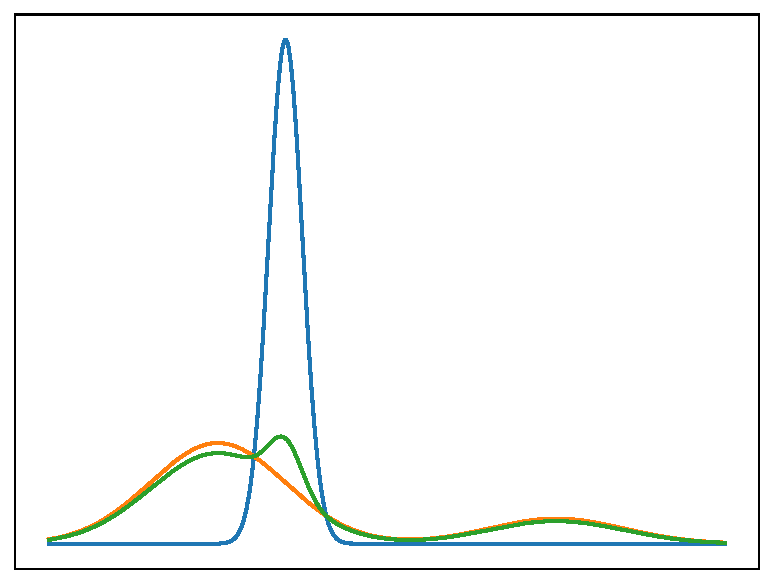
\includegraphics[width = .29\textwidth]{include/figures/1dplotslw5_delta1}
        & 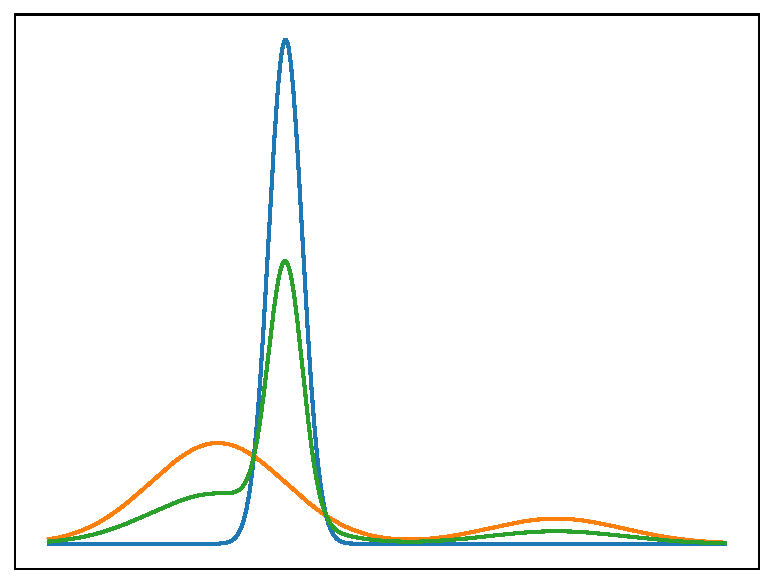
\includegraphics[width = .29\textwidth]{include/figures/1dplotslw5_delta5}
        & 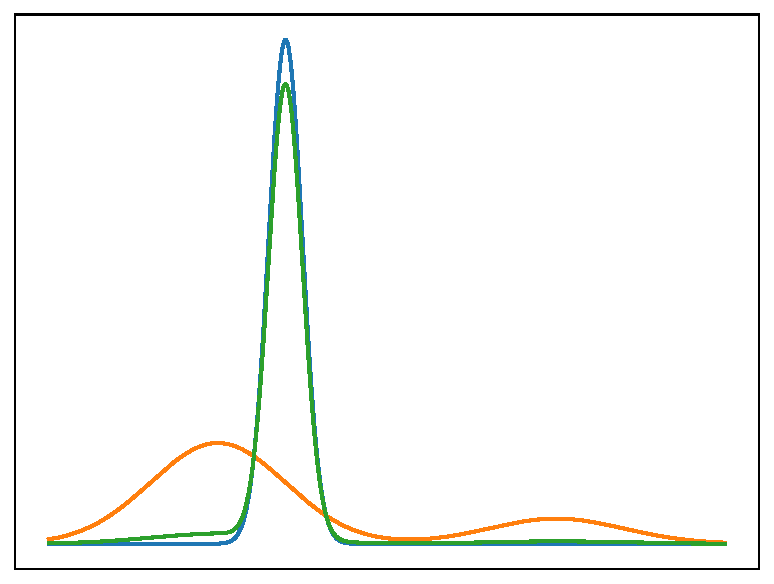
\includegraphics[width = .29\textwidth]{include/figures/1dplotslw5_delta9} \\
        \midrule
        4 & 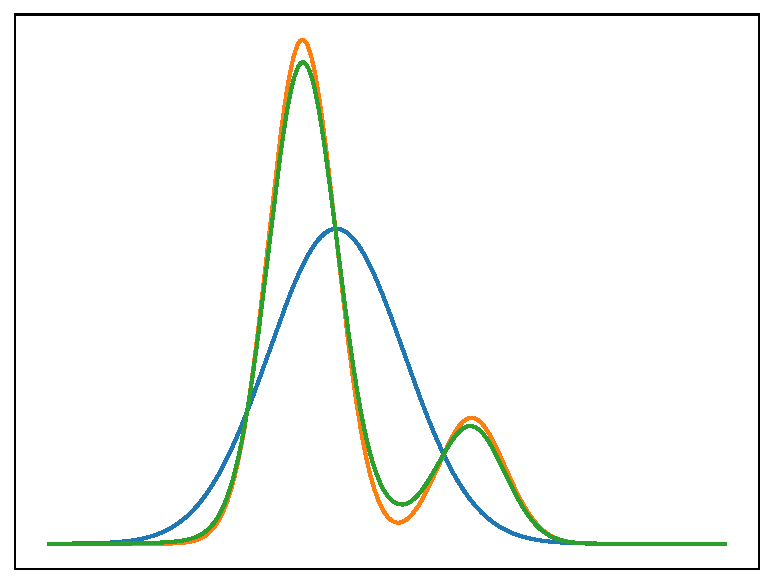
\includegraphics[width = .29\textwidth]{include/figures/1dplotslw40_delta1}
        & 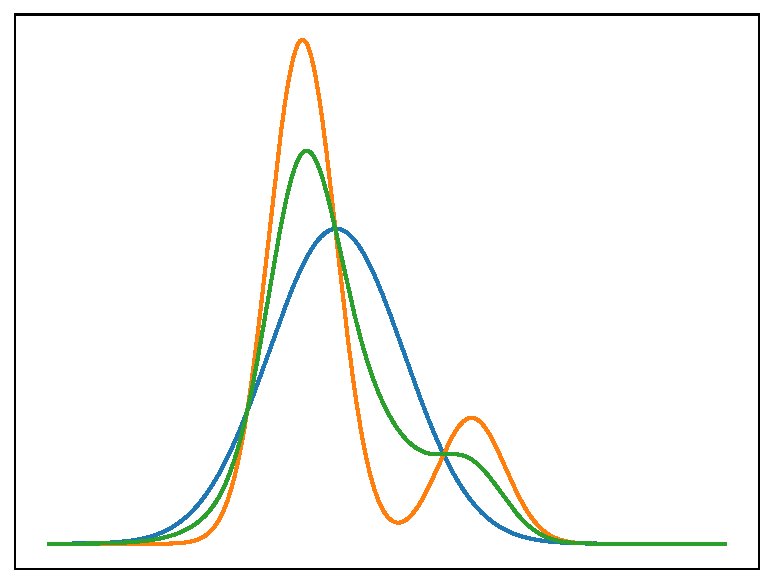
\includegraphics[width = .29\textwidth]{include/figures/1dplotslw40_delta5}
        & 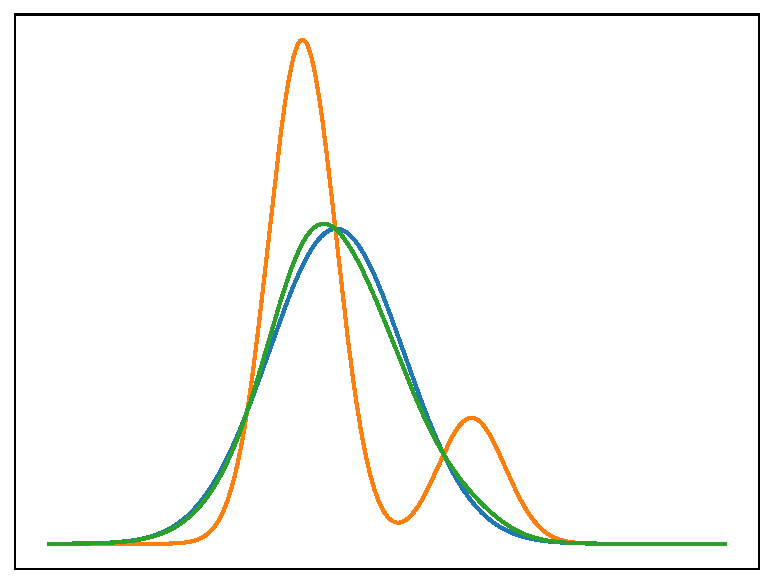
\includegraphics[width = .29\textwidth]{include/figures/1dplotslw40_delta9} \\
        \midrule
        8 & 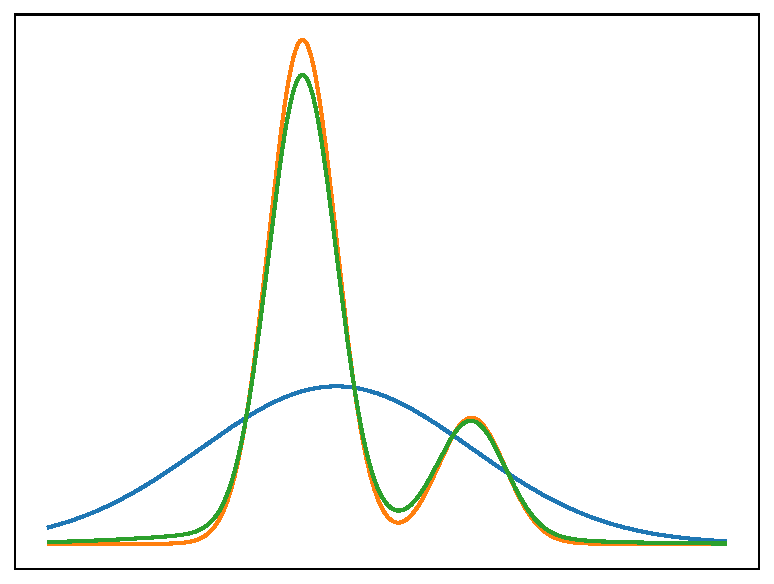
\includegraphics[width = .29\textwidth]{include/figures/1dplotslw80_delta1}
        & 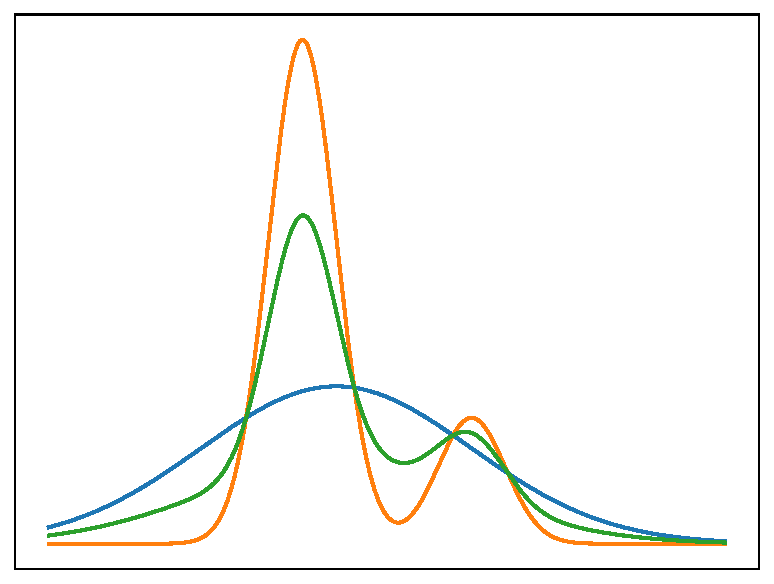
\includegraphics[width = .29\textwidth]{include/figures/1dplotslw80_delta5}
        & 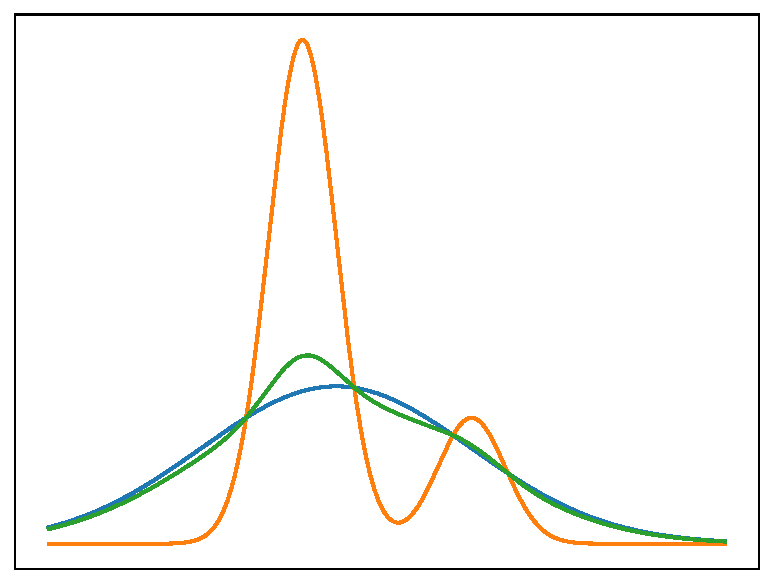
\includegraphics[width = .29\textwidth]{include/figures/1dplotslw80_delta9} \\
        \midrule
        10 & 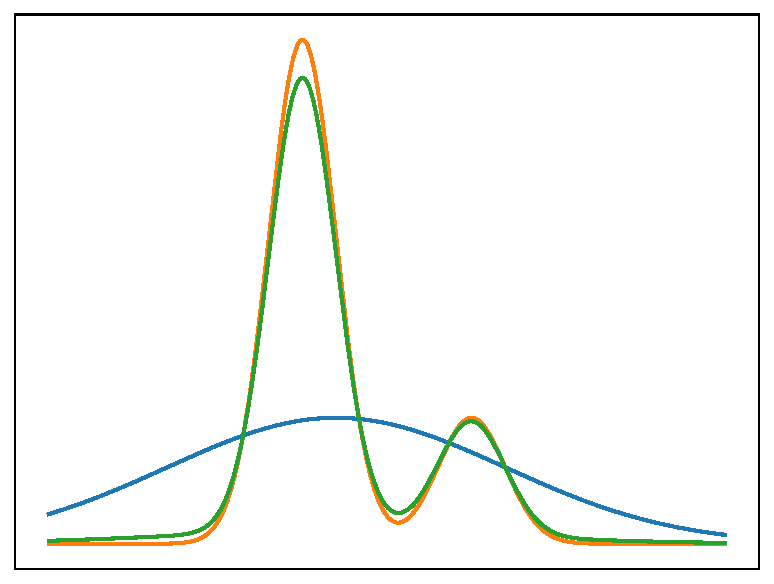
\includegraphics[width = .29\textwidth]{include/figures/1dplotslw100_delta1}
        & 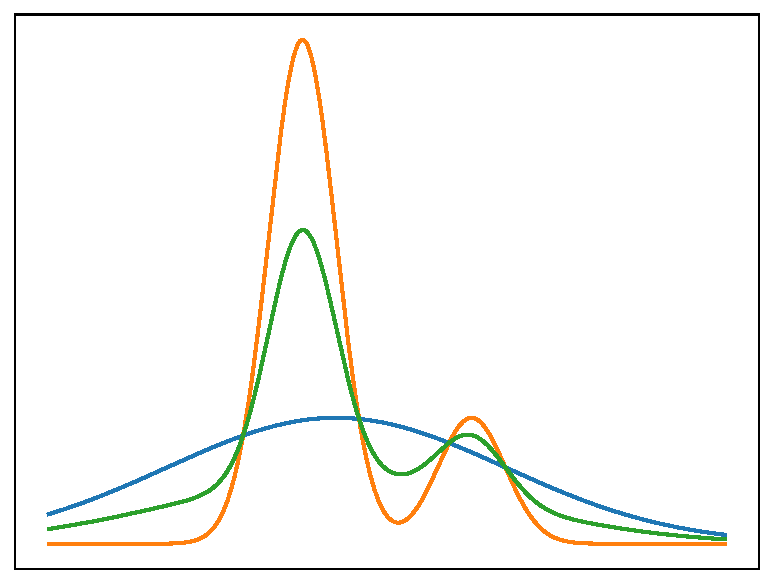
\includegraphics[width = .29\textwidth]{include/figures/1dplotslw100_delta5}
        & 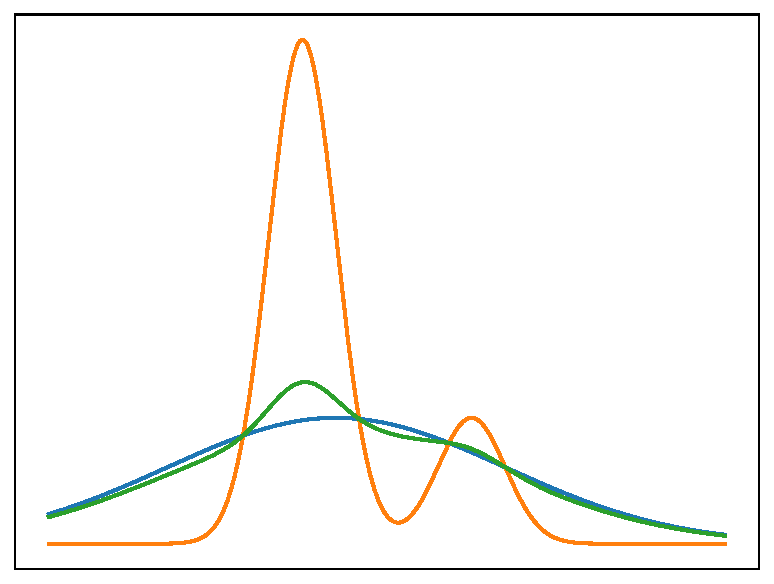
\includegraphics[width = .29\textwidth]{include/figures/1dplotslw100_delta9}
    \end{tabularx}
    \caption{1D Plots for different $\delta$ and $\sigma_{w3}$}
    $w_1 = 5$, $w_2 = -5$, $\alpha = 0.2$, $\sigma_w = 2$.
    The blue plot represents the third normal,
    the orange/red one represents the binormal,
    and the green one represents the mixture.
    The $x$ and $y$ labels and ticks are omitted for clarity.
    \label{tab:1dplotbitri}
\end{table}
\Cref{tab:1dplotbitri} offers a visual representation of how the parameter $\delta$ influences
the shape of the trinormal distribution.
Each plot illustrates \glspl{pdf} for different combinations of $\sigma_{w 3}$
(standard deviation of the third normal distribution) and $\delta$.
The row values in the table correspond to $\sigma_{w 3}$,
while the column values represent $\delta$.
We can observe two key trends within these plots:
\begin{enumerate}
    \item \emph{Influence of $\sigma_{w3}$:}
    As expected, varying $\sigma_{w3}$ primarily affects the \enquote{width}
    or overall variance of the combined distribution.
    When $\sigma_{w3}$ is larger than the width of the original binormal sum (orange/red line),
    choosing a larger $\delta$ allows the overall variance to increase significantly,
    as predicted by \cref{eq:w_prime_2_transform}.

    \item \emph{Decreasing skewness with increasing $\delta$:}
    The plots also reveal a distinct relationship between $\delta$
    and the skewness of the resulting distribution.
    As $\delta$ increases,
    the skewness of the combined trinormal distribution (green line) progressively reduces.
    This phenomenon can be attributed to the placement of the third normal distribution.
    Placed directly between the two original normal distributions,
    the third normal distribution acts as a centralizing force.
    As the weight of the third normal distribution (controlled by $\delta$) grows,
    its symmetric nature counteracts the potential skewness of the initial binormal sum.
    This effect is particularly strong in the bottom three plots,
    where a larger value of $\sigma_{w 3} = 10$ is used.
    We observe a clear reduction in the skewness of the green plot (mixture) as $\delta$ approaches 1.
\end{enumerate}


\section{Deduced lower order moments}\label{sec:dedmoments}

We start by outlining the equations capturing lower-order moments,
expressed in terms of \gls{pdf} parameters.
These equations can be presented in either \emph{dimensional} or \emph{non-dimensional} form.
While both representations are mathematically valid,
the \emph{non-dimensional} form offers a distinct advantage:
it highlights the underlying connection to the bivariate case.

\subsection{Moments for $w$}\label{subsec:lowerordermoments_w}

The relationship for $\overline{w}$ is given as follows:
\begin{align}
    \label{eq:w_bar}
    \overline{w} = (1 - \delta) \alpha w_1 + (1 - \delta)(1-\alpha) w_2 + \delta w_3,
\end{align}
where $w_3 \equiv \alpha w_1 + (1 - \alpha) w_2$.
Therefore the mean of $w$ stays the same as in the bivariate case.
The relationship for the \emph{non-dimensional} form is:
\begin{align}
    \label{eq:w_bar_nondim}
    0 &= \alpha \widehat{w}_1 + (1 - \alpha) \widehat{w}_2
\end{align}
For all other moments -- except for the mean --
we are using the standardized versions of the variables, written as \gls{w_prime}.

The second order moment is given as:
\begin{align}
    \label{eq:wp2_bar}
    \wptwo
    &= (1 - \delta) \alpha [(w_1 - \overline{w})^2 + \sigma_w^2] \nonumber\\
    &+ (1 - \delta) (1 - \alpha) [(w_2 - \overline{w})^2 + \sigma_w^2] \nonumber\\
    &+ \delta \sigma_{w 3}^2,
\end{align}
where $\sigma_{w 3}$ is defined as $\lambda_w \wptwo$.
This moment is also the variance of $w$ at the same time, since
\begin{align*}
    \overline{w'^2}
    &= \mathbb{E}[w'^2]
    = \mathbb{E}[(w - \overline{w})^2]
    = \mathbb{E}[(w - \mathbb{E}[w])^2]
    = \mathbb{E}[w^2 -2w\mathbb{E}[w] + \mathbb{E}[w]^2] \\
    &= \mathbb{E}[w^2] - 2\mathbb{E}[w\mathbb{E}[w]] + \mathbb{E}[\mathbb{E}[w]^2]
    = \mathbb{E}[w^2] - 2\mathbb{E}[w]\mathbb{E}[w] + \mathbb{E}[w]^2 \\
    &= \mathbb{E}[w^2] - \mathbb{E}[w]^2
    = \text{Var}[w].
\end{align*}
The \emph{non-dimensional} relationship would then be:
\begin{align}
    \label{eq:wp2_bar_non_dim}
    \frac{1}{\tswfact}
    &= \alpha \left(\widehat{w}_1^2 + \frac{\tilde{\sigma_w}^2}{(1 - \tilde{\sigma_w})^2} \right)
    + (1-\alpha) \left( \widehat{w}_2^2 + \frac{\tsw^2}{\tswfact} \right).
\end{align}

The third order moment is given as:
\begin{align}
    \label{eq:wp3_bar}
    \wpthree
    &= (1 - \delta) \alpha [(w_1 - \overline{w})^3 + 3 \sigma_w^2 (w_1 - \overline{w})] \nonumber\\
    &+ (1 - \delta) (1 - \alpha) [(w_2 - \overline{w})^3 + 3 \sigma_w^2 (w_2 - \overline{w})]
\end{align}
Since we want to make use of the specific shape of the \gls{pdf},
we also have a relationship for $w'^3$,
which is called $\widehat{Sk}_w$, meaning the skewness of the variable $w$:
\begin{align}
    \widehat{Sk}_w
    &\equiv \frac{1}{\tswfact^{3/2}}
    \frac{\wpthree}{\left( \wptwo \right)^{3/2}}
    \frac{1}{\left(\frac{1-\delta \lambda_w}{1-\delta}\right)^{3/2}}
    \frac{1}{1-\delta} \nonumber \\
    &= \alpha \left(\widehat{w}_1^3 + 3 \widehat{w}_1 \frac{\tsw^2}{\tswfact} \right) +
    (1 - \alpha) \left( \widehat{w}_2^3 + 3 \widehat{w}_2 \frac{\tsw^2}{\tswfact} \right)
    \label{eq:sk_hat_w_nondim}
\end{align}

\subsection{Moments for $\theta_l$}\label{subsec:lowerordermoments_thl}

For $\theta_l$ we have a similar \emph{non-dimensional} relationship:
\begin{align}
    \label{eq:thlp_bar_nondim}
    0 &= \alpha \tilde{\theta}_{l1} + (1 - \alpha) \tilde{\theta}_{l2}
\end{align}
Similarly but with a different standard deviation, $\thlptwo$ is given as:
\begin{align}
    \label{eq:thlp2_bar}
    \thlptwo
    &= (1 - \delta) \alpha [(\theta_{l1} - \overline{\theta_l})^2 + \sigma_{\theta_{l1}}^2] \nonumber\\
    &+ (1 - \delta) (1 - \alpha) [(\theta_{l2} - \overline{\theta_l})^2 + \sigma_{\theta_{l2}}^2] \nonumber\\
    &+ \delta \sigma_{\theta_l 3}^2,
\end{align}
where $\sigma_{\theta_l 3}$ is defined as $\lambda_{\theta_l} \thlptwo$.
This can also be expressed as the variance following the same approach as the one for $\wptwo$.

The third order moment is given as:
\begin{align}
    \label{eq:theta_l_3_bar}
    \thlpthree
    &= (1 - \delta) \alpha [(\theta_{l1} - \overline{\theta_l})^3
    + 3 \sigma_{\theta_{l1}}^2 (\theta_{l1} - \overline{\theta_l})] \nonumber\\
    &+ (1 - \delta) (1 - \alpha) [(\theta_{l2} - \overline{\theta_l})^3
    + 3 \sigma_{\theta_{l2}}^2 (\theta_{l2} - \overline{\theta_l})]
\end{align}
Similarly to \cref{eq:sk_hat_w_nondim}, we also list a moment which is more diagnosed than prognosed:
\begin{align}
    \widehat{Sk_{\theta_l}}
    &\equiv \frac{\thlpthree}{\left(\thlptwo\right)^{3/2}}
    \left(\frac{1}{\frac{1-\delta \lambda_\theta}{1-\delta}}\right)^{3/2}
    \frac{1}{1-\delta} \nonumber\\
    &= \alpha \left( \tilde{\theta}_{l1}^3 + 3 \tilde{\theta}_{l1} \tilde{\sigma}_{\theta_l 1}^2 \right)
    + (1 - \alpha) \left( \tilde{\theta}_{l2}^3 + 3 \tilde{\theta}_{l2} \tilde{\sigma}_{\theta_l 2}^2 \right).
    \label{eq:sk_hat_theta_l_nondim}
\end{align}

\subsection{Moments for $r_t$}\label{subsec:lowerordermoments_rt}

The relationships for $r_t$ and $r_t'^2$ are given as follows
\begin{align}
    \label{eq:rt_bar_nondim}
    0 &= \alpha \tilde{r}_{t1} + (1 - \alpha) \tilde{r}_{t2},
\end{align}
and
\begin{align}
    \label{rtptwo_nondim}
    1 &= \alpha \left( \tilde{r}_{t1}^2 + \tilde{\sigma}_{r_{t1}}^2 \right) +
    (1 - \alpha) \left( \tilde{r}_{t2}^2 + \tilde{\sigma}_{r_{t2}}^2 \right).
\end{align}
Since this relationship is similar to the relationships of $\theta_l$ and $\theta_l'^2$,
we are using nearly the same formulas:
\begin{align}
    \label{eq:r_t_prime_2_bar}
    \rtptwo
    &= (1 - \delta) \alpha [(r_{t1} - \overline{r_t})^2 + \sigma_{r_{t1}}^2] \nonumber\\
    &+ (1 - \delta) (1 - \alpha) [(r_{t2} - \overline{r_t})^2 + \sigma_{\theta_{l2}}^2] \nonumber\\
    &+ \delta \sigma_{r_t 3}^2,
\end{align}
and
\begin{align}
    \label{eq:r_t_prime_3_bar}
    \rtpthree
    &= (1 - \delta) \alpha [(r_{t1} - \overline{r_t})^3 + 3 \sigma_{r_{t1}}^2 (r_{t1} - \overline{r_t})] \nonumber\\
    &+ (1 - \delta) (1 - \alpha) [(r_{t2} - \overline{r_t})^3 + 3 \sigma_{r_{t2}}^2 (r_{t2} - \overline{r_t})]
\end{align}

\subsection{Mixed moments}\label{subsec:lowerordermoments_mixed}

There are also equations for two or even three variables, which are listed in the following.
\begin{align}
    \label{eq:w_prime_theta_l_prime_bar}
    \wpthlp
    &= (1 - \delta) \alpha [(w_1 - \overline{w}) (\theta_{l1} - \overline{\theta_l})] \nonumber\\
    &+ (1 - \delta) (1 - \alpha) [(w_2 - \overline{w}) (\theta_{l2} - \overline{\theta_l})] \nonumber\\
    &+ \delta \lambda_{w\theta} \wpthlp,
\end{align}
\begin{align}
    \label{eq:w_prime_r_t_prime_bar}
    \wprtp
    &= (1 - \delta) \alpha [(w_1 - \overline{w}) (r_{t1} - \overline{r_t})] \nonumber\\
    &+ (1 - \delta) (1 - \alpha) [(w_2 - \overline{w}) (r_{t2} - \overline{r_t})] \nonumber\\
    &+ \delta \lambda_{wr} \wprtp,
\end{align}
and
\begin{align}
    \label{eq:r_t_prime_theta_l_prime_bar}
    \rtpthlp
    &= (1 - \delta) \alpha \left[
        \left(r_{t1} - \overline{r_t}\right)
        \left(\theta_{l1} - \overline{\theta_l}\right) +
        r_{r_t \theta_l} \sigma_{r_{t1}} \sigma_{\theta_{l1}}
        \right] \nonumber\\
    &+ (1 - \delta) (1 - \alpha) \left[
        \left(r_{t2} - \overline{r_t}\right)
        \left(\theta_{l2} - \overline{\theta_l}\right) +
        r_{r_t \theta_l} \sigma_{r_{t2}} \sigma_{\theta_{l2}}
        \right] \nonumber\\
    &+ \delta \lambda_{r\theta} \overline{r_t' \theta_l'}.
\end{align}
We have the \emph{non-dimensional} relationship for those moments given as
\begin{align}
    \widehat{c}_{w \theta_l}
    &\equiv \frac{1}{\tswfact^{1/2}}
    \frac{\overline{w' \theta_l'}}{\sqrt{\wptwo}\sqrt{\thlptwo}}
    \frac{1}{\sqrt{\frac{1 - \delta \lambda_w}{1 - \delta}}}
    \frac{1}{\sqrt{\frac{1 - \delta \lambda_\theta}{1 - \delta}}}
    \frac{1 - \delta \lambda_{w\theta}}{1 - \delta} \nonumber\\
    &= \alpha \widehat{w}_1 \tilde{\theta}_{l1} +
    (1 - \alpha) \widehat{w}_2 \tilde{\theta}_{l2},
    \label{eq:c_hat_w_theta_l_nondim}
\end{align}
\begin{align}
    \widehat{c}_{w r_t}
    &\equiv \frac{1}{\tswfact^{1/2}}
    \frac{\overline{w' r_t'}}{\sqrt{\wptwo}\sqrt{\rtptwo}}
    \frac{1}{\sqrt{\frac{1 - \delta \lambda_w}{1 - \delta}}}
    \frac{1}{\sqrt{\frac{1 - \delta \lambda_r}{1-\delta}}}
    \frac{1 - \delta \lambda_{w r}}{1-\delta} \nonumber\\
    &= \alpha \widehat{w}_1 \tilde{r}_{t1} +
    (1 - \alpha) \widehat{w}_2 \tilde{r}_{t2},
    \label{eq:c_hat_w_r_t_nondim}
\end{align}
and
\begin{align}
    \widehat{c}_{r_t \theta_l}
    &\equiv \frac{\rtpthlp}{\sqrt{\rtptwo}\sqrt{\thlptwo}}
    \frac{1}{\sqrt{\frac{1-\delta \lambda_q}{1-\delta}}}
    \frac{1}{\sqrt{\frac{1-\delta \lambda_\theta}{1-\delta}}}
    \frac{1 - \delta \lambda_{\theta r} }{1 - \delta} \nonumber\\
    &= \alpha \left(\tilde{r}_{t1} \tilde{\theta}_{l1} +
    r_{r_t \theta_l} \tilde{\sigma}_{q_{t1}} \tilde{\sigma}_{\theta_{l1}} \right) +
    (1 - \alpha) \left(\tilde{r}_{t2} \tilde{\theta}_{l2} +
    r_{r_t \theta_l} \tilde{\sigma}_{r_{t2}} \tilde{\sigma}_{\theta_{l2}} \right),
    \label{eq:c_hat_r_t_theta_l_nondim}
\end{align}
where we can think about $\widehat{c}$ as the correlation.

We also list a trivariate moment ($\wprtpthlp$), given by:
\begin{align}
    \wprtpthlp
    &= (1 - \delta) \alpha (w_1 - \overline{w}) \left[
        \left(r_{t1} - \overline{r_t}\right)
        \left(\theta_{l1} - \overline{\theta_l}\right) +
        r_{r_t \theta_l} \sigma_{r_{t1}} \sigma_{\theta_{l1}}
        \right] \nonumber\\
    &+ (1 - \delta) (1 - \alpha) (w_2 - \overline{w}) \left[
        \left(r_{t2} - \overline{r_t}\right)
        \left(\theta_{l2} - \overline{\theta_l}\right) +
        r_{r_t \theta_l} \sigma_{r_{t2}} \sigma_{\theta_{l2}}
    \right].
    \label{eq:w_prime_r_t_prime_t_l_prime_bar}
\end{align}

\section{Finding pdf parameters in terms of moments}\label{sec:pdfparams}

We now select a particular member of the normal mixture family
by mapping the prognosed moments to the \gls{pdf} parameters.
In other words, we invert \cref{eq:w_bar_nondim} - \cref{eq:c_hat_r_t_theta_l_nondim}
in order to find the set of \gls{pdf} parameters
that guarantees that the resulting \gls{pdf} has moments that correspond to the prognosed ones.
The inversion is non-trivial because the equations are non-linear in the \gls{pdf} parameters.
However, the \gls{pdf} (\cref{eq:normal_mix_pdf}) is simple enough to permit an analytic solution.

The solution procedure is as follows.
\begin{enumerate}
    \item Solve for the \gls{pdf} parameters $\alpha$, $\widehat{w}_1$,
    and $\widehat{w}_2$ from the moment equations for $\overline{w}$ (\cref{eq:w_bar_nondim}),
    $\wptwo$ (\cref{eq:wp2_bar_non_dim}), $\wpthree$ (\cref{eq:sk_hat_w_nondim}):
    \begin{align}
        \label{eq:alpha_solved}
        \alpha
        &= \frac{1}{2}\left[1 - \widehat{Sk}_w \sqrt{\frac{1}{4 + \widehat{Sk}_w^2}}\right],
    \end{align}
    \begin{align}
        \label{eq:w1_solved}
        \widehat{w}_1
        &= \sqrt{\frac{1-\alpha}{\alpha}},
    \end{align}
    \begin{align}
        \label{eq:w2_solved}
        \widehat{w}_2
        &= -\sqrt{\frac{\alpha}{1-\alpha}}.
    \end{align}
    Without loss of generality, it has been chosen to set $\widehat{w}_1 > \widehat{w}_2$.

    \item \Cref{eq:alpha_solved} implies that $\widehat{Sk}_w$ is determined solely by $\alpha$:
    \begin{align}
        \label{eq:sk_w_alpha}
        \widehat{Sk}_w
        &= \frac{1-2\alpha}{\sqrt{\alpha(1-\alpha)}}.
    \end{align}

    \item We can obtain $\Tilde{\theta}_{l1}$ and $\Tilde{\theta}_{l2}$ from \cref{eq:thlp_bar_nondim}
    for $\overline{\theta_l}$, and \cref{eq:c_hat_w_theta_l_nondim} for $\wpthlp$:
    \begin{align}
        \label{eq:thl1_tilde_solved}
        \tilde{\theta}_{l1}
        &= -\frac{\widehat{c}_{w \theta_l}}{\widehat{w}_2},
    \end{align}
    \begin{align}
        \label{eq:thl2_tilde_solved}
        \tilde{\theta}_{l2}
        &= -\frac{\widehat{c}_{w \theta_l}}{\widehat{w}_1}.
    \end{align}

    \item The widths of the normals, $\tilde{\sigma}_{\theta_l 1}$ and $\tilde{\sigma}_{\theta_l 2}$,
    are determined by satisfying \cref{eq:thlp2_bar} for $\thlptwo$,
    and \cref{eq:theta_l_3_bar} for $\thlpthree$:
    \begin{align}
        \label{eq:sigma_tilde_theta1_solved}
        \tilde{\sigma}_{\theta_l 1}^2
        &= \left(1-\widehat{c}_{w \theta_l}^2 \right) +
        \left(\sqrt{\frac{1 - \alpha}{\alpha}}\right)
        \frac{1}{3 \widehat{c}_{w \theta_l}}
        \left( \widehat{Sk_{\theta_l}} - \widehat{c}_{w \theta_l}^3 \widehat{Sk}_w \right),
    \end{align}
    \begin{align}
        \label{eq:sigma_tilde_theta2_solved}
        \tilde{\sigma}_{\theta_l 2}^2
        &= \left(1 - \widehat{c}_{w \theta_l}^2 \right) -
        \left(\sqrt{\frac{\alpha}{1 - \alpha}}\right)
        \frac{1}{3 \widehat{c}_{w \theta_l}}
        \left( \widehat{Sk_{\theta_l}} - \widehat{c}_{w \theta_l}^3 \widehat{Sk}_w \right).
    \end{align}
    Here $Sk_{\theta_l}$ is the skewness of $\theta_l$.
    It must be provided either by a prognostic equation or by a diagnostic equation
    such as \cref{eq:sk_hat_theta_l_nondim} below.

    \item Equations for $\tilde{r}_{t1}$, $\tilde{r}_{t2}$, $\tilde{\sigma}_{r_t 1}^2$,
    and $\tilde{\sigma}_{r_t 2}^2$ are found by expressions identical to \cref{eq:thl1_tilde_solved},
    \cref{eq:thl2_tilde_solved}, \cref{eq:sigma_tilde_theta1_solved},
    and \cref{eq:sigma_tilde_theta2_solved}, except that $\theta_l$ is replaced everywhere by $r_t$.

    \item Finally, from \cref{eq:r_t_prime_theta_l_prime_bar} for $\rtpthlp$ we find
    \begin{align}
        \label{eq:r_r_t_theta_l}
        r_{r_t \theta_l}
        &= \frac{\widehat{c}_{r_t \theta_l} - \widehat{c}_{w r_t} \widehat{c}_{w \theta_l}}
        {\alpha \tilde{\sigma}_{r_{t}1}\tilde{\sigma}_{\theta_{l}1} +
            (1-\alpha) \tilde{\sigma}_{r_{t}2} \tilde{\sigma}_{\theta_{l}2}}.
    \end{align}
    Here $r_{r_t \theta_l}$ is the in-between normal correlation and $c_{r_t \theta_l}$
    is the total correlation.
\end{enumerate}

\section{Leveraging the pdf for higher-order moment calculations}
\label{sec:leveraging-the-pdf-for-higher-order-moment-calculations}

Upon determining the \gls{pdf} parameters,
we gain the ability to compute all higher-order moments associated with the distribution.
These moments play a crucial role for closing the already described \glspl{pde}.
The symbolic calculation of higher-order moments can be achieved
through integration over the specified \gls{pdf}.
Formulas for calculating various higher-order moments within the context of a binormal \gls{pdf}
are readily available in the literature~\cite{larson2005using}.

We state the transformed formulas needed for closure in the following.

\begin{align}
    \label{eq:wp4_div_wp2_2}
    \frac{1}{\tswfact^2} \frac{(1-\delta)}{(1-\delta \lambda_w)^2} \frac{\wpfour}{\left(\wptwo \right)^2}
    &= \alpha \left[\widehat{w}_1^4 +
    6 \widehat{w}_1^2 \frac{\tsw^2}{\tswfact} +
    3 \frac{\tsw^4}{\tswfact^2} \right] \nonumber \\
    &+ (1 - \alpha) \left[\widehat{w}_2^4 +
    6 \widehat{w}_2^2 \frac{\tsw^2}{\tswfact} +
    3 \frac{\tsw^4}{\tswfact^2} \right] \nonumber \\
    &+ \frac{1}{\tswfact^2} \frac{(1-\delta)}{(1-\delta \lambda_w)^2} \delta 3 \lambda_w^2,
\end{align}
\begin{align}
    \label{eq:wp2thlp_div_wp2thl2}
    \frac{1}{\tswfact} \frac{(1-\delta)^{1/2}}{(1-\delta \lambda_w) (1-\delta \lambda_\theta)^{1/2}}
    \frac{\wptwothlp}{\wptwo \left(\thlptwo \right)^{1/2}}
    &= \alpha \left[\widehat{w}_1^2 + \frac{\tsw^2}{\tswfact} \right] \tilde{\theta}_{l1} \nonumber\\
    &+ (1-\alpha) \left[\widehat{w}_2^2 + \frac{\tsw^2}{\tswfact}\right] \tilde{\theta}_{l2},
\end{align}
\begin{align}
    \label{eq:wpthlp2_div_wp2_thlp2}
    \frac{1}{\tswfact^{1/2}} \frac{(1-\delta)^{1/2}}{(1-\delta \lambda_w)^{1/2} (1-\delta \lambda_\theta)}
    \frac{\wpthlptwo}{\left(\wptwo\right)^{1/2}\thlptwo}
    = \alpha  \widehat{w}_1  \left( \tilde{\theta}_{l1}^2 + \tilde{\sigma}_{\theta_{l1}}^2 \right)
    + (1-\alpha) \widehat{w}_2 \left( \tilde{\theta}_{l2}^2 + \tilde{\sigma}_{\theta_{l2}}^2 \right),
\end{align}
\begin{align}
    \label{eq:wprtpthlp_div_wp2_thp2_rt2}
    \frac{1}{\tswfact^{1/2}}
    \frac{(1-\delta)^{1/2}}
    {(1-\delta \lambda_w)^{1/2} (1-\delta \lambda_\theta)^{1/2}(1-\delta \lambda_{q_t})^{1/2}}
    \frac{\wprtpthlp}
    {\left( \wptwo \right)^{1/2}\left(\rtptwo \right)^{1/2} \left( \thlptwo \right)^{1/2}} \nonumber \\
    = \alpha \widehat{w}_1 \left(\tilde{r}_{t1} \tilde{\theta}_{l1} +
    r_{r_t \theta_l} \tilde{\sigma}_{r_{t1}} \tilde{\sigma}_{\theta_{l1}} \right) +
    (1-\alpha) \widehat{w}_2 \left(\tilde{r}_{t2} \tilde{\theta}_{l2} +
    r_{r_t \theta_l} \tilde{\sigma}_{r_{t2}} \tilde{\sigma}_{\theta_{l2}} \right)
\end{align}
Equations for $\wptwortp$ and $\wprtptwo$ are similar to \cref{eq:wp2thlp_div_wp2thl2}
and \cref{eq:wpthlp2_div_wp2_thlp2} by replacing $\theta_l$ with $r_t$ everywhere.

\section{A diagnostic ansatz for the skewness of heat and moisture}\label{sec:diag_ansatz}

We cannot close the system of equations until we specify the skewness of $\theta_l$, $Sk_{\theta_l}$, that appears in \cref{eq:sigma_tilde_theta1_solved} for $\tilde{\sigma}_{\theta_l 1}$, and \cref{eq:sigma_tilde_theta2_solved} for $\tilde{\sigma}_{\theta_l 2}$.
Likewise, we need to specify $Sk_{r_t}$.
We could prognose these scalar skewnesses, but this would involve additional computational expense, storage, and complexity.
In some cases, the extra complexity may be worthwhile.
However, here we instead propose the following diagnostic formula
\begin{align}
    \label{eq:Sk_hat_thl_beta}
    \widehat{Sk}_{\theta_l}
    &= \widehat{Sk}_w \widehat{c}_{w \theta_l} \left[\beta + (1-\beta) \widehat{c}_{w \theta_l}^2 \right],
\end{align}

and a similar formula for $\widehat{Sk}_{r_t}$.
The parameter $\beta$ is dimensionless.
We also solve for $\beta$ because we are going to need the equation later on to show that other equations are true.
\begin{align}
    \label{eq:beta}
    \implies \beta
    &=\frac{\frac{\widehat{Sk}_{\theta_l}}{\widehat{Sk}_w \widehat{c}_{w \theta_l}} - \widehat{c}_{w \theta_l}^2}{1 - \widehat{c}_{w \theta_l}^2}
\end{align}
\Cref{eq:Sk_hat_thl_beta} is physically plausible but limited at the same time.
The formula states that $Sk_{\theta_l}$ is proportional to $Sk_w$, the skewness of $w$.
An increase in $\beta$ leads to an increase in $\left| Sk_{\theta_l} \right|$, which, in turn, leads to a \gls{pdf} with a longer $\theta_l$-tail.
$Sk_{\theta_l}$ and $Sk_w$ have the same sign when $w$ and $\theta_l$ are positively correlated;
$Sk_{\theta_l}$ and $Sk_w$ have opposite sign when $w$ and $\theta_l$ are negatively correlated.
In those large eddy simulations, this is usually but not always true.
$Sk_{\theta_l}$ vanishes when either $Sk_w$ or $c_{w \theta_l}$ vanishes;
clearly this need not be true in nature.
$\left| Sk_{\theta_l} \right|$ can be either smaller or larger than $\left| Sk_w \right|$, depending on the values of $\tsw^2$, $c_{w \theta_l}$, and $\beta$.

If we assume our ansatz (\cref{eq:sk_hat_theta_l_nondim}) for $\widehat{Sk}_{\theta_l}$, then the $\theta_l$-widths of the first (\cref{eq:sigma_tilde_theta1_solved}) and secondnormal(\cref{eq:sigma_tilde_theta1_solved}) reduce to
\begin{align}
    \label{eq:sigma_theta1_beta}
    \tilde{\sigma}_{\theta_l 1}^2
    &= \frac{\left(1 - \widehat{c}_{w \theta_l}^2\right)}{\alpha} \left[\frac{1}{3} \beta + \alpha \left(1 - \frac{2}{3} \beta\right)\right],
\end{align}

and
\begin{align}
    \label{eq:sigma_theta2_beta}
    \tilde{\sigma}_{\theta_l 2}^2
    &= \frac{\left(1 - \widehat{c}_{w \theta_l}^2\right)} {1 - \alpha} \left\{1 - \left[\frac{1}{3}\beta + \alpha \left(1 - \frac{2}{3} \beta \right)\right]\right\}.
\end{align}

Substituting \cref{eq:sigma_theta1_beta}, \cref{eq:sigma_theta2_beta}, and their $r_t$ counterparts into the expression for $r_{r_t \theta_l}$ \cref{eq:r_r_t_theta_l} yields the simplified form:
\begin{align}
    \label{eq:r_r_t_theta_l_beta}
    r_{r_t \theta_l}
    &= \frac{c_{r_t \theta_l} - \widehat{c}_{w r_t} \widehat{c}_{w \theta_l}}{\left(1 - \widehat{c}_{w r_t}^2\right)^{1/2} \left(1 - \widehat{c}_{w \theta_l}^2\right)^{1/2}}.
\end{align}

Here, $r_{r_t \theta_l}$ is the correlation of $r_t$ and $\theta_l$ in-between the Normals and $c_{r_t \theta_l}$ is the total correlation.

\gls{CLUBB} chose a specific formula for the $w$-\enquote{width} of the individual Gaussians, which is the following:
\begin{align}
    \label{eq:sigma_tilde_w_restricted}
    \tsw^2
    &= \gamma \left[1 - \max(c_{w \theta_l}^2, c_{w r_t}^2) \right].
\end{align}
This makes $\tsw^2$ depend on $c_{w r_t}^2$ and $c_{w \theta_l}^2$.
Here $0 \leq \gamma < 1$ is a dimensionless constant.
This formula helps ensure that when $c_{w r_t}$ or $c_{w \theta_l}$ becomes large in magnitude, $0 \leq \widehat{c}_{w \theta_l}^2, \widehat{c}_{w r_t}^2 < 1$ and hence $\tilde{\sigma}_{r_t 1,2}^2$, $\tilde{\sigma}_{\theta_l 1,2}^2$, and $r_{r_t \theta_l}$ remain realistic.

\section{Proposed closures for third- and fourth-order moments based on the mixture of trivariate normals}
\label{sec:prop_closure}

This section lists formulas for the higher-order moments that are needed for closure
in the parameterization of $\wpfour$, $\wptwothlp$, $\wpthlptwo$, and $\wprtpthlp$.
These are obtained by substituting the expressions for the \gls{pdf} parameters
(\cref{eq:alpha_solved} - \cref{eq:r_r_t_theta_l}) into the equations for the higher-order moments
(\cref{eq:wp4_div_wp2_2} - \cref{eq:wprtpthlp_div_wp2_thp2_rt2}).
Formulas for $\wptwortp$ and $\wprtptwo$,
which are also needed,
are identical to those for $\wptwothlp$ and $\wpthlptwo$ except that $r_t$ replaces $\theta_l$ everywhere.

First, we list the equation for $\theta_l'^3$, which is obtained by dimensionalizing \cref{eq:Sk_hat_thl_beta}:
\begin{align}
    \label{eq:thlp3_beta}
    \overline{\theta_l'^3}
    &= \frac{(1-\delta \lambda_{w \theta})(1-\delta \lambda_\theta)}{\tswfact^2 (1-\delta \lambda_w)^2}
    \frac{\overline{w'^3}}{\left( \overline{w'^2} \right)^2}
    \overline{\theta_l'^2} \;
    \overline{w'\theta_l'}
    \left(\beta + (1-\beta)
    \frac{(1-\delta \lambda_{w \theta})^2}{1-\tilde{\sigma}_w^2 (1-\delta \lambda_w)(1-\delta \lambda_\theta)}
    \frac{\left(\overline{w'\theta_l'}\right)^2}{\overline{w'^2} \; \overline{\theta_l'^2}}\right).
\end{align}
While the scalar third moments are not essential for solving the prognostic equations directly,
they still play a role in shaping cloud properties.
This is because cumulus clouds tend to form at the edges,
or \enquote{tails}, of the \gls{pdf} for a specific variable.
Typically, as the relative \enquote{width} of the normal distribution in $w$
(represented by $\tsw^2=\sigma_w^2/\wptwo$) increases,
the value of $\thlpthree$ also grows (see \cref{eq:thlp3_beta}) for details).
In simpler terms,
a larger $\thlpthree$ corresponds to a broader $w$-marginal \gls{pdf},
which deviates further from a double delta function (a function with two spikes at zero).

$\wpfour$ does not depend on the thermodynamic scalar moments;
therefore, it does not depend on $\beta$.
Substituting \cref{eq:w1_solved} and \cref{eq:w1_solved} into \cref{eq:wp4_div_wp2_2}
and using \cref{eq:sk_hat_w_nondim}, we find
\begin{align}
    \label{eq:wp4_div_wp2_2_solved}
    \frac{1}{\tswfact^2} \frac{(1-\delta)}{(1-\delta \lambda_w)^2} \frac{\wpfour}{\left(\wptwo\right)^2}
    &= 3 \frac{\tsw^4}{\tswfact^2} + 6 \frac{\tsw^2}{\tswfact} + 1 \nonumber\\
    &+ \widehat{Sk}_w^2 + \frac{1}{\tswfact^2} \frac{(1-\delta)}{(1-\delta \lambda_w)^2} \delta 3 \lambda_w^2,
\end{align}
and also
\begin{align}
    \label{eq:wp4}
    \overline{w'^4}
    &= \left(\overline{w'^2}\right)^2
    \frac{(1-\delta \lambda_w)^2}{(1-\delta)}
    \left(3 \tilde{\sigma}_w^4 + 6 \tswfact \tilde{\sigma}_w^2 + \tswfact^2\right) \nonumber\\
    &+ \frac{1}{\tswfact} \frac{1}{(1-\delta \lambda_w)}
    \frac{\left(\overline{w'^3}\right)^2}{\overline{w'^2}} \nonumber\\
    &+ \delta 3 \lambda_w^2 \left(\overline{w'^2}\right)^2.
\end{align}
Similar to $\wpfour$, $\wptwothlp$ does not depend on $\beta$ for our particular \gls{pdf} family.
Substituting \cref{eq:w1_solved} - \cref{eq:thl2_tilde_solved} into \cref{eq:wp2thlp_div_wp2thl2},
we find
\begin{align}
    \label{eq:wp2thlp_sk_w_solved}
    \frac{1}{\tswfact} \frac{(1-\delta)^{1/2}}{(1-\delta \lambda_w) (1-\delta \lambda_\theta)^{1/2}} \frac{\overline{w'^2\theta_l'}}{\overline{w'^2} \left(\overline{\theta_l'^2} \right)^{1/2}}
    &= \widehat{c}_{w\theta_l} \widehat{Sk}_w,
\end{align}
and
\begin{align}
    \label{eq:wp2thlp_solved}
    \overline{w'^2\theta_l'}
    &= \frac{1}{\tswfact} \frac{1 - \delta \lambda_{w\theta}}{1-\delta \lambda_w} \frac{\overline{w'^3}}{\overline{w'^2}} \overline{w'\theta_l'}.
\end{align}
$\wpthlptwo$ depends explicitly on $Sk_{\theta_l}$.
Substituting \cref{eq:w1_solved} - \cref{eq:sigma_tilde_theta2_solved}
into \cref{eq:wprtpthlp_div_wp2_thp2_rt2} yields
\begin{align}
    \label{eq:wpthlp2_sk_w_solved}
    \frac{1}{\tswfact^{1/2}} \frac{(1-\delta)^{1/2}}{(1-\delta \lambda_w)^{1/2} (1-\delta \lambda_\theta)} \frac{\overline{w'\theta_l'^2}}{\left(\overline{w'^2}\right)^{1/2} \overline{\theta_l'^2}}
    &= \frac{2}{3} \widehat{c}_{w\theta_l}^2 \widehat{Sk}_w + \frac{1}{3} \frac{ \widehat{Sk_{\theta_l}} } {\widehat{c}_{w\theta_l}},
\end{align}
and
\begin{align}
    \label{eq:wpthlp2_solved}
    \overline{w'\theta_l'^2}
    &= \frac{2}{3} \frac{(1-\delta \lambda_{w \theta})^2}{(1-\delta \lambda_w)^2} \frac{1}{\tswfact^2} \frac{\overline{w'^3}}{\left(\overline{w'^2} \right)^2} \left(\overline{w'\theta_l'} \right)^2 \nonumber\\
    &+ \frac{1}{3} \frac{(1-\delta \lambda_w)}{(1-\delta \lambda_{w \theta})} \tswfact \frac{\overline{w'^2} \; \overline{\theta_l'^3} }{\overline{w'\theta_l'}}.
\end{align}
The formula has a problem because $\wpthlp$ is in the denominator.
As $\wpthlp$ gets closer to zero, the formula becomes infinitely large, which is called a singularity.
This can cause issues if we use the formula directly with real-world measurements of $\thlpthree$ and $\wpthlp$.
The resulting diagnosis of $\wpthlptwo$ would be very sensitive to small changes in the measurements
and might not be reliable (noisy).
We can fix this singularity by either
\begin{itemize}
    \item substitute in the ansatz for $Sk_{\theta_l}$ (\cref{eq:sk_hat_theta_l_nondim})
    into the original formula (\cref{eq:wpthlp2_div_wp2_thlp2}),
    \item or, equivalently, substitute \cref{eq:thlp3_beta} for $\thlpthree$.
    This is possible because \cref{eq:thlp3_beta} shows that $\thlpthree$ is proportional to $\wpthlp$.
\end{itemize}
Both approaches effectively remove the singularity from the formula.
Therefore, we find:
\begin{align}
    \label{eq:wpthlp2_div_wp2_thlp2_sk_w}
    \frac{1}{\tswfact^{1/2}} \frac{(1-\delta)^{1/2}}{(1-\delta \lambda_w)^{1/2} (1-\delta \lambda_\theta)} \frac{\overline{w'\theta_l'^2}}{\left(\overline{w'^2}\right)^{1/2} \overline{\theta_l'^2}}
    &= \widehat{Sk}_w \left[\frac{1}{3} \beta + \left(1 - \frac{1}{3} \beta \right) \widehat{c}_{w\theta_l}^2 \right],
\end{align}
and
\begin{align}
    \label{eq:wpthlp2_beta}
    \overline{w'\theta_l'^2}
    &= \frac{1}{\tswfact} \frac{(1-\delta \lambda_\theta)}{(1-\delta \lambda_w)}
    \frac{\overline{w'^3}}{\overline{w'^2}}
    \left[ \frac{1}{3} \beta \overline{\theta_l'^2}
    + \frac{\left( 1-\frac{1}{3} \beta \right)}{\tswfact}
    \frac{(1-\delta \lambda_{w \theta})^2}{(1-\delta \lambda_w)(1-\delta \lambda_\theta)}
    \frac{\left( \overline{w'\theta_l'} \right)^2}{\overline{w'^2}}
    \right].
\end{align}
Finally, substituting \cref{eq:w1_solved} - \cref{eq:r_r_t_theta_l} into \cref{eq:wprtpthlp_div_wp2_thp2_rt2}
yields the following formula for the turbulent flux of $\rtpthlp$, $\wprtpthlp$:
\begin{align}
    \label{eq:wprtpthlp_div_wp2_thp2_rt2_sk_w}
    \frac{(1-\delta)^{1/2}}{(1-\delta \lambda_w)^{1/2}
        (1-\delta \lambda_\theta)^{1/2}
        (1-\delta \lambda_{r_t})^{1/2}}
    \frac{\wprtpthlp}{\tswfact^{1/2}
        \left( \overline{w'^2} \right)^{1/2}
        \left(\rtptwo\right)^{1/2} \left(\thlptwo\right)^{1/2}} \nonumber \\
    = \widehat{c}_{wr_t} \widehat{c}_{w\theta_l} \widehat{Sk}_w
    + E(w,q_t,\theta_l) \frac{1}{2} \widehat{Sk}_w
    \left( c_{q_t\theta_l} - \widehat{c}_{wr_t} \widehat{c}_{w\theta_l}\right),
\end{align}
and
\begin{align}
    \label{eq:wprtpthlp_E}
    \wprtpthlp
    &= \frac{\frac{1}{2} E}{\tswfact}
    \frac{(1-\delta \lambda_{\theta q})} {(1 - \delta \lambda_w)}
    \rtpthlp \frac{\overline{w'^3}}{\overline{w'^2}} \nonumber\\
    &+ \frac{1 - \frac{1}{2} E}{\tswfact^2}
    \frac{(1-\delta \lambda_{w q})(1-\delta \lambda_{w \theta})}{(1 - \delta \lambda_w)^2}
    \wprtp \; \wpthlp \frac{\overline{w'^3}}{\left( \overline{w'^2} \right)^2}.
\end{align}
The function $E(w,r_t,\theta_l)$ is
\begin{align}
    \label{eq:E}
    E &= \frac{1 - \frac{1}{2} \frac{2\alpha}{1-2\alpha} \xi}{1 + \frac{1}{2} \xi},
\end{align}
where
\begin{align}
    1 + \xi
    = \frac{1-\alpha}{\alpha} \frac{\tilde{\sigma}_{r_{t2}}}{\tilde{\sigma}_{r_{t1}}} \frac{ \tilde{\sigma}_{\theta_{l2}}}{\tilde{\sigma}_{\theta_{l1}}}
    = \left(\frac{A_{r_t} - B_{r_t}}{-A_{r_t} - B_{r_t}}\right)^{1/2} \left(\frac{A_{\theta_l} - B_{\theta_l}}{-A_{\theta_l} - B_{\theta_l}}\right)^{1/2},
\end{align}
and
\begin{align}
    \label{eq:A_thl}
    A_{\theta_l}
    &= Sk_{\theta_l} - \frac{3}{2} \widehat{c}_{w\theta_l} \widehat{Sk}_w + \frac{1}{2} \widehat{c}_{w\theta_l}^3 \widehat{Sk}_w,
\end{align}
\begin{align}
    B_{\theta_l}
    &= \frac{3}{2} \left(4 + \widehat{Sk}_w^2 \right)^{1/2} \widehat{c}_{w\theta_l} \left(1 - \widehat{c}_{w\theta_l}^2\right),
\end{align}
and $A_{r_t}$ and $B_{r_t}$ are analogous.
We now list two cases in which the expression for $E$ simplifies.
First, if
\begin{align*}
    \frac{\tilde{\sigma}_{r_{t2}}}{\tilde{\sigma}_{r_{t1}}} \frac{\tilde{\sigma}_{\theta_{l2}}}{\tilde{\sigma}_{\theta_{l1}}}
    &= 1
\end{align*}
then $E=0$.
This would occur, for instance,
if the \enquote{widths} of the first and second normal were equal to each other for both $r_t$ and $\theta_l$,
that is, if $\tilde{\sigma}_{r_{t2}} = \tilde{\sigma}_{r_{t1}}$
and $\tilde{\sigma}_{\theta_{l2}} = \tilde{\sigma}_{\theta_{l1}}$.
Second, if we use the diagnostic ansatz (\cref{eq:sk_hat_theta_l_nondim}) for the scalar skewnesses, then
\begin{align}
    \label{eq:xi}
    \xi = \frac{1 - 2 \zeta}{\zeta},
\end{align}
where
\begin{align}
    \label{eq:zeta}
    \zeta = \alpha + \frac{1}{3} \beta \left(1 - 2 \alpha \right).
\end{align}

Then we find
\begin{align}
    \label{eq:E_eq_23beta}
    E &= \frac{2}{3} \beta,
\end{align}
and finally
\begin{align}
    \label{eq:wpqtpthlp_beta}
    \wprtpthlp
    &= \frac{\frac{1}{3}\beta}{\tswfact}
    \frac{(1-\delta \lambda_{\theta r})}{(1 - \delta \lambda_w)}
    \rtpthlp \frac{\overline{w'^3}}{\overline{w'^2}} \nonumber\\
    &+ \frac{1 - \frac{1}{3}\beta}{\tswfact^2}
    \frac{(1-\delta \lambda_{w r})(1-\delta \lambda_{w \theta})} {(1 - \delta \lambda_w)^2}
    \wprtp \; \wpthlp \frac{\overline{w'^3}}{\left( \overline{w'^2} \right)^2}.
\end{align}